\chapter{Teoretická část}
\section{Charakteristika časových řad}
Časové řady představují sekvence datových bodů, které jsou zaznamenávány buď v pravidelných intervalech v čase, nebo kontinuálně. 
V případě, že jsou hodnoty měřeny v konkrétních a oddělených časových okamžicích, hovoříme o diskrétní časové řadě.
Naopak, pokud lze veličinu považovat za definovanou v každém okamžiku času, jedná se o kontinuální časovou řadu.

Tyto datové body mohou představovat různé jevy, například teplotní záznamy, údaje z finančních trhů, senzorová měření, dopravní intenzitu, spotřebu energie nebo jiné sledované hodnoty. 
Nemusejí však být nutně číselné, mohou být také kategorické, například stav zařízení nebo typ události.
Datové body také nemusejí být striktně naměřené v přesný okamžik, ale mohou představovat agregované hodnoty za určitý časový interval,
například denní průměrnou teplotu nebo hodinový výstup pracovní linky. Délka těchto intervalů se volí podle povahy sledovaného jevu a požadavků analýzy a může sahat od sekund až po měsíce či roky.
\cite{diggle2025time}

\subsection{Analýza}
V podstatě všechny časové řady jsou zaznamenávány za účelem následné analýzy. Tato analýza může mít různé cíle, které lze shrnout do následujících kategorií:
\begin{enumerate}
  \item \textbf{Zkoumání vlivů na sledovaný jev} \\
  Časové řady se často používají k odhalování vztahů mezi různými faktory a sledovaným jevem. 
  Například v ekonomii mohou být analyzovány dopady změn úrokových sazeb na inflaci nebo v energetice vliv teploty na spotřebu elektrické energie. 
  Taková analýza umožňuje pochopit, jak jednotlivé vlivy ovlivňují chování systému v čase.
  \item \textbf{Studium samotného jevu} \\
  Někdy je cílem zkoumat pouze samotný jev.
  Například meteorologické časové řady teplot mohou odhalit dlouhodobé oteplování, sezónní výkyvy nebo extrémní jevy, jako jsou vlny horka.
  \item \textbf{Predikce budoucího vývoje} \\
  Historická data umožňují předpovídat budoucí hodnoty sledovaného jevu. 
  Taková predikce se využívá například při plánování kapacit výroby, řízení zásob nebo finančních investic.
\end{enumerate} 

Analýza časových řad zahrnuje různé techniky a metody, které umožňují identifikovat vzory, trendy, sezónní výkyvy a další charakteristiky v datech.
\cite{diggle2025time}

\begin{figure}[H]
        \centering
        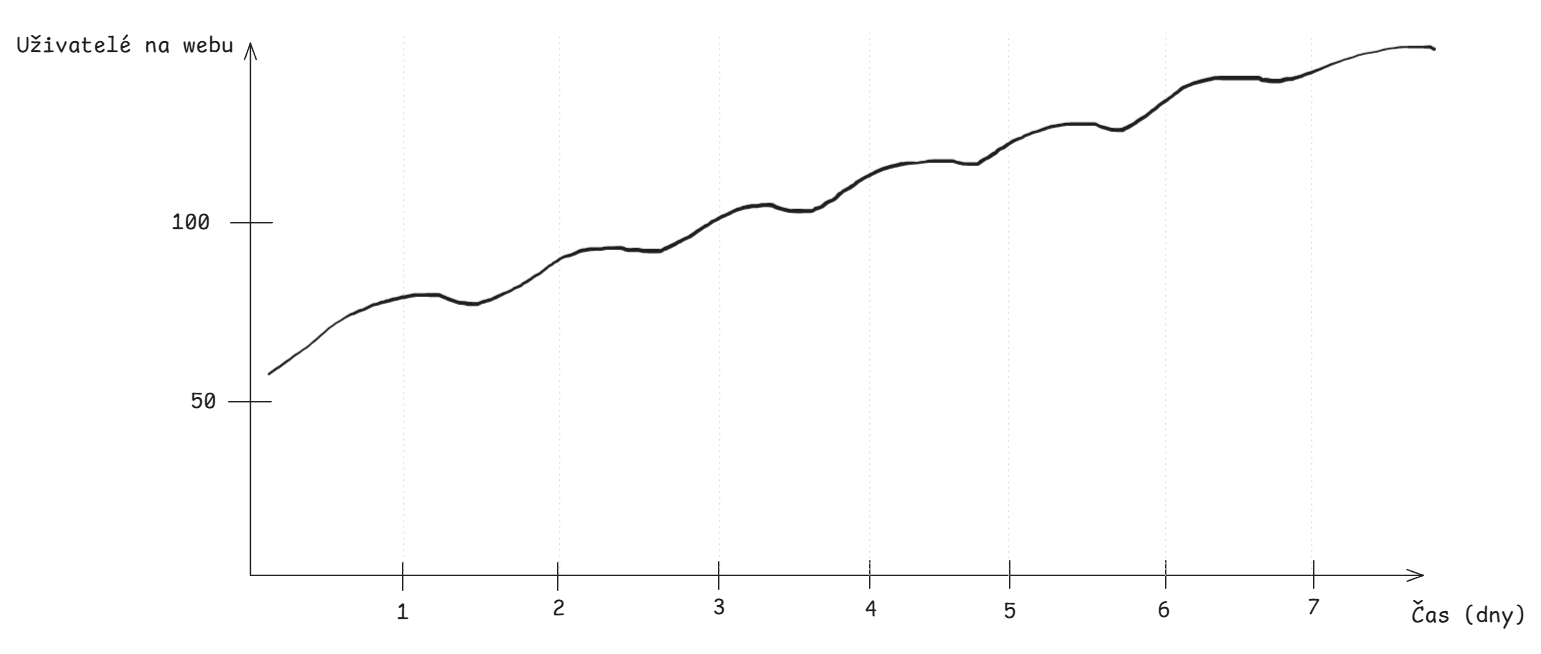
\includegraphics[width=0.8\textwidth]{images/casova_rada.png}
        \caption{Ukázka časové řady}
        \label{fig:casova_rada}
\end{figure}
Na obrázku \ref{fig:casova_rada} je znázorněna ukázka časové řady, kde na vodorovné ose jsou zobrazeny časové okamžiky v rámci dní a na svislé ose hodnoty sledovaného jevu - Současných online uživatelů na webovém portálu.

Lze na ní pozorovat denní cyklus, neboli sezónnost, kdy počet uživatelů vrcholí v odpoledních hodinách a klesá během noci, a zároveň linární rostoucí trend, stránku každý den navštíví více uživatelů.

% \subsection{Historie časových řad}
% Studium časových řad má dlouhou historii, sahající až do starověkých civilizací, kde byly zaznamenávány astronomické jevy a zemědělské cykly.

% \subsubsection{Medicína}
% Jedna z prvních zaznamenaných časových řad oblasti medicíny pochází od jistého Johna Graunta, prodejce klobouků, který v 17. století studoval záznamy úmrtí v Londýně
% a následně vydal knížku Natural and Political Observations Made upon the Bills of Mortality. V této knížce prezentoval "life tables", 
% tabulky které ukazovaly pravděpodobnost úmrtí před dalšimi narozeninami v různých věkových kategoriích.

\section{Ukládání časových řad}
Mnohdy hodnota časových řad leží spíše v retrospektivní analýze než v analyzování každé nové hodnoty v reálném čase.
Z tohoto důvodu je často potřeba tyto časové řady efektivně ukládat pro pozdější analýzu.
Existuje mnoho různých přístupů k ukládání časových řad, od tradičních relačních databází přes specializované databázové systémy navržené speciálně pro tento účel
až po obyčejné textové soubory.

Při výběru správného formátu a databázového systému pro ukládání časových řad je důležité zvážit několik faktorů, jako jsou:
\begin{itemize}
    \item \textbf{Objem dat} \\ 
    Časové řady mohou a mnohdy i generují daleko větší objemy dat než jiné typy dat. Tento objem je důležité předem odhadnout a
    zvolit systém, který je schopný efektivně tento růst zvládnout.
    \item \textbf{Neustálý příjem nebo jednotlivé události} \\
    Při vybírání ideálního systému, například pro ukládání návštěvnosti webových stránek, je potřeba zvážit charakter dat.  
    V případě neustálého toku dat je obvykle nejzajímavější pracovat s nejnovějšími záznamy, protože ty starší mohou být méně relevantní pro analýzu.  
    Naopak pokud data představují jednotlivé události, například každoroční dopravní provoz během svátků, může být důležité mít přístup i k historickým datům. 
    V takovém případě je pravděpodobnější, že systém bude potřebovat podporu pro náhodný přístup k různým časovým intervalům.
    \item \textbf{Trvání projektu} \\
    Pokud je projekt krátkodobý, může být dostačující použít jednodušší a rychle nasaditelná řešení, jako jsou textové soubory nebo jednoduché databáze.
    Pokud známe délku projektu, daleko snáze se odhaduje objem dat, který bude potřeba uložit.
    \item \textbf{Zpracování a životní cyklus dat} \\ 
    Je vhodné předem stanovit, jak budou data zpracovávána a jak dlouho mají být uchovávána.  
    Ne všechny záznamy je nutné uchovávat trvale, některé lze po určité době agregovat, 
    downsamplovat\footnote{\textit{Downsampling} - proces převzorkování dat na menší počet datových bodů} nebo smazat.  
    Definování jasné strategie mazání či archivace dat pomáhá předejít nekontrolovatelnému růstu databáze a zároveň usnadňuje správu a optimalizaci výkonu systému.  
\end{itemize}    

Tyto faktory pomohou určit, jestli je nutné ukládat neupravená data nebo předem zpracovaná.

\subsection{Životnost dat}
Při rozhodování o tom, jaké úložiště dat je vhodné, je klíčové porozumět životnímu cyklu dat. 
Čím realističtější budeme ohledně skutečného využití dat, tím méně jich je nutné ukládat a tím méně času strávíme hledáním ideálního úložného systému. 
Mnoho organizací zaznamenává příliš mnoho událostí a bojí se o ztrátu dat, ale mít obrovské množství špatně zpracovatelných dat 
je mnohem méně užitečné než mít agregovaná data uložená v relevantních časových intervalech.

U krátkodobých dat, například výkonnostních metrik, které se sledují jen kvůli ověření, že je vše v pořádku, možná vůbec nebude 
potřeba ukládat data v původní podobě, nebo alespoň ne na dlouho. To je zvlášť důležité u dat založených na událostech, kde jednotlivé 
události samy o sobě nejsou významné a hlavní hodnotu mají až souhrnné statistiky. \cite{nielsen2019practical}

Předpokládejme, že sledujeme dobu načítání webové stránky v sekundách.
V tabulce \ref{table:1} je uvedena ukázka časové řady načítání webové stránky v různých časových okamžicích.
\begin{table}[ht!]
\centering
\begin{tabular}{||c | c||} 
    \hline
    \textbf{Časové razítko} & \textbf{Čas načtení stránky} \\ [0.5ex] 
    \hline\hline
    Duben 5, 2024 10:22:24 & 23s \\ 
    \hline
    Duben 5, 2024 10:22:28 & 15s \\
    \hline
    Duben 5, 2024 10:22:41 & 14s \\
    \hline
    Duben 5, 2024 10:23:02 & 11s \\
    \hline
    Duben 5, 2024 10:23:15 & 19s \\
    \hline
    Duben 5, 2024 10:23:33 & 12s \\
    \hline
\end{tabular}
\caption{Časová řada načítání webové stránky}
\label{table:1}
\end{table}

V takovém případě nás nezajímá každý jednotlivý záznam, ale spíše souhrnné statistiky, jako je průměrný čas načítání za minutu, hodinu nebo den.
Proto můžeme zvolit strategii, kde budeme uchovávat pouze agregovaná data, například průměrný čas načítání za každou minutu, a původní záznamy po určité době smazat.
Tímto způsobem můžeme výrazně snížit objem uložených dat a zároveň zachovat relevantní informace pro analýzu výkonu webové stránky. \cite{nielsen2019practical}

Výsledný záznam by tedy mohl vypadat například takto v tabulce \ref{table:2}.
\begin{table}[ht!]
\centering
\begin{tabular}{||c | c | c | c | c||} 
    \hline
    \textbf{Časové rozmezí} & \textbf{Prům. čas načtení} & \textbf{Počet přístupů} & \textbf{Min. čas} & \textbf{Max. čas} \\ [0.5ex] 
    \hline\hline
    Duben 5, 2024 10:00:00 & 15.6s & 6 & 11s & 19s \\ 
    \hline
    Duben 5, 2024 11:00:00 & 17.2s & 4 & 9s & 25s \\
    \hline
\end{tabular}
\caption{Zjednodušený záznam časové řady načítání webové stránky}
\label{table:2}
\end{table}


\section{Databázové systémy}
Databázové systémy jsou ten nejběžnější způsob jak ukládat časové řady.  Většinou jsou připravené tzv. "out of the box", neboli ihned po pořízení, 
poskytují spoustu vestavěných funkcí pro jednoduché zpracování dat, jako je například agregace a filtrování.
Navíc jsou optimalizované pro rychlý zápis a čtení dat, a dokáží škálovat s rostoucím objemem dat. \cite{nielsen2019practical}

\subsection{SQL a NoSQL databáze}
Hlavní rozdíl mezi SQL a NoSQL databázemi spočívá v jejich struktuře a způsobu ukládání dat. [\cite{microsoftnosql}]

%upravit ještě
\begin{itemize}
    \item[\textbf{SQL}] 
    SQL databáze jsou relační databáze, které používají strukturovaný dotazovací jazyk (SQL) pro správu a manipulaci s daty.
    Data jsou organizována do tabulek s pevně definovanými schématy, což znamená, že každá tabulka má předem stanovené sloupce a datové typy.
    Tento přístup je vhodný, když předem známe strukturu dat a víme, že se nebude měnit. \cite{microsoftsql}
    \begin{figure}[H]
        \centering
        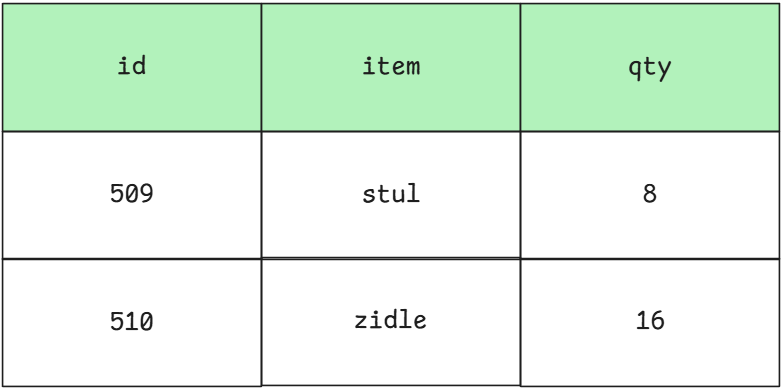
\includegraphics[width=0.8\textwidth]{images/sql_example.png}
        \caption{Ukázka struktury SQL databáze}
        \label{fig:sql_example}
    \end{figure}

    \item[\textbf{NoSQL}] 
    NoSQL databáze naopak nabízejí flexibilnější přístup k ukládání dat.
    Nejsou vázány na pevná schémata a umožňují ukládání dat v různých formátech, ty nejčastěji používané jsou:
\end{itemize}

\begin{itemize}
    \item \textbf{Databáze párů klíč-hodnota} \\ 
    Ukládají data jako páry klíč-hodnota, což umožňuje rychlý přístup k datům na základě klíče. Používá se v případech,
    kdy struktura klíčů je známá, ale hodnoty mohou být různého typu nebo formátu.

    Jeden z nejznámějších příkladů je Redis, který je často využíván pro 
    caching\footnote{\textit{Caching} - technika ukládání často používaných dat do rychlé paměti} a real-time aplikace jakožto 
    dodatečná vrstva mezi uživatelem a koncovou databází. \cite{redisusecases}

    \begin{lstlisting}[caption={Redis - ukázka syntaxe}, label={lst:redis}, captionpos=b]
    HSET `user:001` first_name `Jan` dob 12-JUN-1970
    (integer) 2

    HGETALL `user:001`
    `first_name`
    `Jan`
    `dob`
    `12-JUN-1970`
    \end{lstlisting}
    \begin{figure}[H]
        \centering
        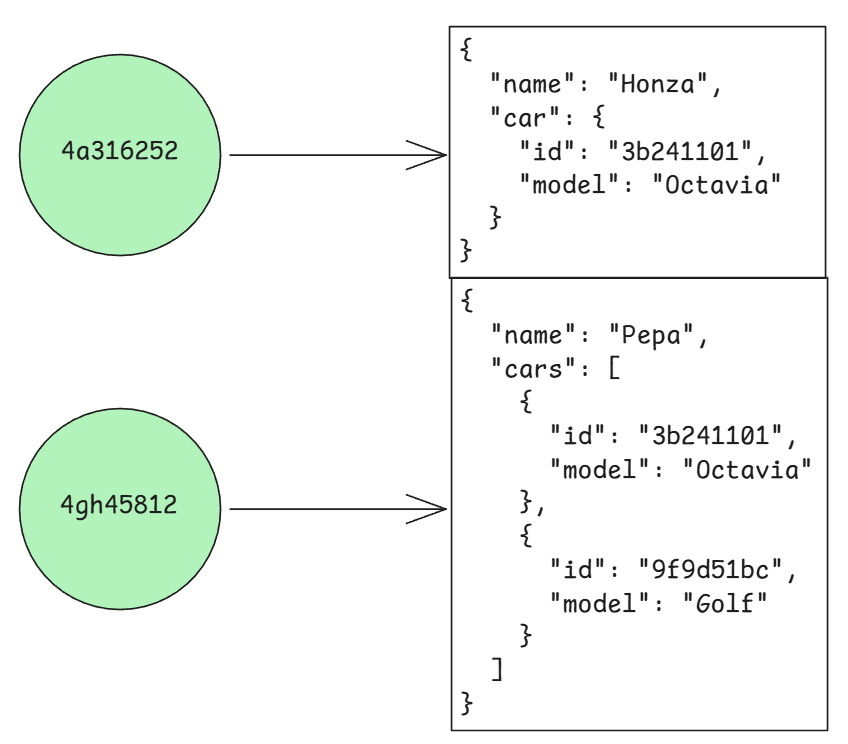
\includegraphics[width=0.8\textwidth]{images/key_value_example.png}
        \caption{Ukázka struktury databáze párů klíč-hodnota}
        \label{fig:key_value_example}
    \end{figure}

    \item \textbf{Databáze dokumentů} \\ 
    Ukládají data ve formě dokumentů, často ve formátu JSON nebo BSON. Každý dokument může mít odlišnou strukturu, což umožňuje větší flexibilitu.
    Větší skupiny dokumentů mohou být organizovány do kolekcí.
    Podporují vnořené páry klíč-hodnota.

    Nejznámější příklad je MongoDB. Často se používá pro webové aplikace, analytické systémy nebo logování, kde se struktura dat může často měnit. \cite{mongodbusecases}
    \begin{lstlisting}[caption={MongoDB - ukázka syntaxe}, label={lst:mongodb}, captionpos=b]
    db.inventory.insertOne(
        { 
            name: `Jan`, 
            dob: new Date(`1970-06-12`) 
        }
    )

    db.inventory.find({ name: `Jan` }).pretty()
    {
        _id: ObjectId(`64f8e9a1b1234567890abcd1`),
        name: `Jan`,
        dob: ISODate(`1970-06-12T00:00:00Z`)
    }
    \end{lstlisting}

    \item \textbf{Databáze sloupců} \\ 
    Ukládají data podle sloupců namísto řádků, což je výhodné pro analytické dotazy, které často pracují s velkým množstvím dat v konkrétních sloupcích.
    Výhoda je v tom že to eliminuje potřebu číst nepotřebná data, což zvyšuje výkon dotazů.

    Jeden z nejznámějších příkladů je ClickHouse, který je často využíván pro analytické úlohy v reálném čase, jako je sledování metrik a logování. \cite{clickhouseusecases}
    \begin{lstlisting}[caption={ClickHouse - ukázka syntaxe}, label={lst:clickhouse}, captionpos=b]
    INSERT INTO water_levels.sensor_readings (sensor_id, location, timestamp, water_level) VALUES
    (201, `River A`, now(), 2.35);

    SELECT sensor_id, location, timestamp, water_level
    FROM water_levels.sensor_readings;
   +-----------+-------------+---------------------+-------------+
    | sensor_id | location    | timestamp           | water_level |
    +-----------+-------------+---------------------+-------------+
    | 201       | River A     | 2025-11-18 12:34:56 | 2.35        |
    +-----------+-------------+---------------------+-------------+
    \end{lstlisting}
    
    \item \textbf{Grafová databáze} \\ 
    Ukládají data jako uzly a hrany, což je ideální pro reprezentaci a analýzu vztahů mezi daty. 
    Uzly představují entity, zatímco hrany reprezentují vztahy mezi nimi.

    Nejznámější příklad je Neo4j, který se často používá pro sociální sítě, doporučovací systémy a analýzu podvodů. \cite{neo4jusecases}
    \begin{figure}[H]
        \centering
        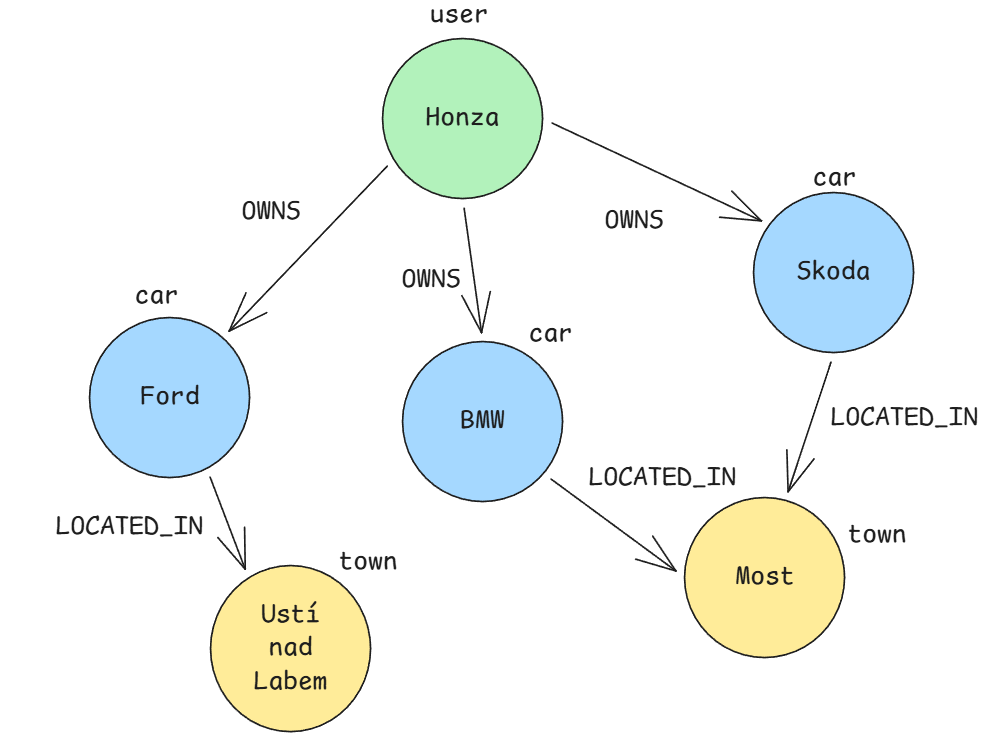
\includegraphics[width=0.8\textwidth]{images/graph_example.png}
        \caption{Ukázka struktury grafové databáze}
        \label{fig:graph_example}
    \end{figure}
    \begin{lstlisting}[caption={Neo4j - ukázka syntaxe}, label={lst:neo4j}, captionpos=b]
    CREATE (jan:Person {name: `Jan`})
    CREATE (eva:Person {name: `Eva`})

    MATCH (jan:Person {name: `Jan`})
    MATCH (eva:Person {name: `Eva`})
    CREATE (jan)-[:KNOWS]->(eva)

    MATCH (jan:Person {name: `Jan`})-[:KNOWS]->(friend)
    RETURN jan.name AS Jan, friend.name AS Knows

    Jan  | Knows
    -----|------
    Jan  | Eva
    \end{lstlisting}

\end{itemize}

\section{Úvod do problematiky testování a implementace}
\subsection{LXC}
LXC je rozhraní uživatelského prostoru pro funkce jádra Linuxu umožňující izolaci procesů.
Díky API a jednoduchým nástrojům umožňuje vytvářet a spravovat systémevé nebo aplikační kontejnery. \cite{lxcintro}

\subsection{LXD}
LXD slouží jako alternative k LXC a poskytuje uživatelsky přívětivější rozhraní pro správu kontejnerů.
Interně ovšem také používá zakládní API LXC. Je doporučený hlavně pro méně zkušené uživatele. 

\subsubsection{Kontejner}
Kontejner představuje standardizovanou softwarovou jednotku, která zapouzdřuje kód aplikace společně se všemi jejími závislostmi a knihovnami. 
Na rozdíl od virtuálních strojů kontejnery neobsahují vlastní operační systém a nevyužívají hypervizor. 
Místo toho sdílejí jádro hostitelského systému, což zajišťuje izolaci procesů při zachování minimální režie. 
Díky tomu jsou kontejnery výrazně menší (často v řádech megabajtů) a jejich spuštění je rychlejší. \cite{redhatcontainers}

Klíčovou vlastností kontejnerů je jejich přenositelnost. Aplikaci zabalenou v kontejneru lze snadno přesouvat mezi různými 
prostředími – od lokálního vývoje až po produkční nasazení v cloudu – s jistotou, že bude fungovat konzistentně bez ohledu na podkladovou 
infrastrukturu. O masivní rozšíření a standardizaci této technologie se v posledních letech zasloužila především platforma Docker.

\subsubsection{Virtuální stroj}
Virtuální stroj je softwarová emulace fyzického počítače, která spouští vlastní kompletní operační systém v izolovaném prostředí. 
Provoz více virtuálních strojů na jednom fyzickém serveru umožňuje vrstva zvaná hypervizor, která se stará o přidělování 
hardwarových prostředků (CPU, paměť, úložiště) jednotlivým instancím. \cite{redhatcontainers}
Hypervizory lze rozdělit do dvou hlavních kategorií:
\begin{itemize}
    \item \textbf{Bare-metal} \\
    Běží přímo na fyzickém hardwaru hostitelského serveru bez prostřednictví operačního systému. Díky přímému přístupu k hardwarovým 
    prostředkům je velmi efektivní a nabízí vysoký výkon, což z něj činí standardní volbu pro podniková datová centra a cloudová prostředí. 
    Mezi známé zástupce patří VMware ESXi, Microsoft Hyper-V nebo KVM (Kernel-based Virtual Machine), který je součástí jádra Linuxu.

    \item \textbf{Hosted} \\
    Instaluje jako běžná softwarová aplikace na již existující operační systém (tzv. hostitelský OS). Hardwarové zdroje jsou 
    virtuálním strojům přidělovány prostřednictvím tohoto hostitelského systému, což zvyšuje režii a mírně snižuje výkon. Tento 
    typ se nejčastěji využívá na osobních počítačích pro vývoj, testování nebo výuku. Typickými příklady jsou Oracle VirtualBox nebo VMware Workstation.
\end{itemize}

Ačkoliv jsou virtuální stroje náročnější na systémové zdroje než kontejnery, poskytují silnou úroveň izolace a 
umožňují provozovat aplikace vyžadující odlišné operační systémy na stejném hardwaru. Historicky stály VM u zrodu cloud computingu a 
dodnes hrají klíčovou roli při konsolidaci serverů, optimalizaci využití hardwaru a v případech, kdy je vyžadována plná virtualizace prostředků.

\section{Ansible}
Ansible je open-source \footnote{\textit{Open-source} - software, jehož zdrojový kód je volně dostupný pro uživatele k prohlížení, úpravám a distribuci.} 
nástroj pro automatizaci IT úloh, jako je konfigurace systémů, nasazení aplikací a správa infrastruktury. 
Na rozdíl od mnoha jiných automatizačních nástrojů nevyžaduje Ansible instalaci agentů \footnote{\textit{Agent} - proces instalovaný na cílovém uzlu, který přijímá instrukce od řídicího serveru, vykonává je a zpětně odesílá stav nebo výsledky} na cílové stroje – komunikuje s 
nimi typicky přes protokol SSH, což výrazně zjednodušuje jeho nasazení i údržbu. \cite{hochstein2017ansible}

Ansible se připojí na cílový uzel přes určitý protokol a nahraje tam dočasný program, nazvaný \texttt{Ansible module}, který vykoná požadované úlohy a poté se sám odstraní.

Ansible byl vytvořen v roce 2012 Michaelem DeHaanem, známým také jako autorem nástrojů Cobbler a Func. Jeho cílem bylo nabídnout 
jednodušší a přístupnější alternativu k tehdejším nástrojům, které vyžadovaly složitější architekturu a používání agentů a 
zároveň poskytnout lepší možnost než jen jednorázový skript pro danou úlohu.

V roce 2015 Ansible získala společnost Red Hat, což přineslo projektu silnou podporu a další rozvoj. Pod vedením Red Hatu se Ansible
 stal jedním z nejpoužívanějších automatizačních nástrojů v podnikovém prostředí a stal se klíčovou součástí širší platformy Red Hat Automation. \cite{hochstein2017ansible}

\subsubsection{Idempotence}
Ansible se snaží být idempotentní, což znamená, že opakované spuštění stejného playbooku by mělo vést k stejnému výsledku bez ohledu 
na to, kolikrát je spuštěn. Né vždy je to ale možné, například při generování náhodných hesel nebo při práci s časově závislými daty.

\subsubsection{Deklarativní přístup}
Ansible umožňuje uživatelům popisovat cílový stav zařízení, nikoli jednotlivé kroky, jak tohoto stavu dosáhnout. Tyto kroky jsou v pozadí
zajišťovány moduly. Může se ale stát, že uživatel bude chtít provést nějakou akci, pro kterou žádný modul neexistuje. 
V takovém případě je možné použít modul \texttt{command} nebo \texttt{shell}, kdy uživatel přímo specifikuje příkaz, který se má na cílovém uzlu spustit. 
\cite{hochstein2017ansible}

\subsubsection{Čitelnost a jednoduchost}
Konfigurace a úlohy jsou zapisovány v jazyce YAML, který je navržen tak, aby byl snadno čitelný a srozumitelný i pro ty, 
kteří nejsou odborníky na programování, tzv. sebedokumentující se jazyk. \cite{hochstein2017ansible}

\subsection{Základní architektura}
\begin{itemize}
    \item \textbf{Řídicí uzel} \\
    Řidící uzel je stroj, na kterém je nainstalován Ansible a odkud jsou spouštěny všechny automatizační úlohy.
    Obsahuje veškeré konfigurační soubory, playbooky a inventáře cílových uzlů. \cite{ansibledocs}

    \item \textbf{Řízené uzly} \\
    Řízené uzly jsou servery nebo zařízení, která Ansible spravuje. Mohou to být například fyzické servery, virtuální stroje, kontejnery nebo síťová zařízení.
    
    Ansible komunikuje s těmito uzly hlavně pomocí protokolu SSH a provádí na nich definované úlohy.
    Existují ale i jiné způsoby komunikace, například \texttt{local} pro lokální operace nebo \texttt{docker} pro správu Docker kontejnerů. \cite{ansibledocs}
    
    V Ansible se dá připojit ať už k jednomu nebo více řízeným uzlům najednou. Pokud není specifikováno jinak, tak paralelně. 
    Tyto skupiny jsou definovány v inventáři.
    \item \textbf{Úloha} \\
    Úloha je základní jednotka práce v Ansible, která definuje konkrétní akci, kterou má Ansible provést na řízeném uzlu.
    Úlohy jsou definovány v playboocích a mohou zahrnovat různé operace, jako je instalace softwaru, kopírování souborů, 
    spouštění příkazů nebo konfigurace služeb. \cite{ansibledocs}
    \begin{lstlisting}[language=YAML, caption={Ansible - ukázka úlohy}, label={lst:ansibletask}, captionpos=b]
    - name: Ensure postgresql is at the latest version
      ansible.builtin.yum:
        name: postgresql
        state: latest
    \end{lstlisting}

    \item \textbf{Playbooky} \\
    Playbooky jsou soubory ve formátu YAML, které obsahují sadu úloh pro Ansible.
    Definují, jaké úlohy mají být provedeny na kterých řízených uzlech a v jakém pořadí.
    Playbooky umožňují automatatizovat složité procesy a zajišťují opakovatelnost a konzistenci konfigurací. \cite{ansibledocs}
    \begin{lstlisting}[language=YAML, caption={Ansible - ukázka playbooku}, label={lst:ansibleplaybook}, captionpos=b]
    ---
    - name: Update db servers
      hosts: dbservers
      remote_user: root

      tasks:
        - name: Ensure postgresql is at the latest version
          ansible.builtin.yum:
            name: postgresql
            state: latest

        - name: Ensure that postgresql is started
          ansible.builtin.service:
            name: postgresql
            state: started
    \end{lstlisting}


    \item \textbf{Moduly} \\
    Moduly představují základní vykonávací jednotky v Ansible. Každá úloha (\textit{task}) v playbooku využívá některý 
    modul k provedení konkrétní operace na řízeném uzlu. Modul tedy definuje, jaký typ akce má být vykonán.
    
    Ansible obsahuje velké množství vestavěných modulů, které jsou dostupné v tzv. \textit{kolekcích}. 
    Nejčastěji používané vestavěné moduly se nacházejí v kolekci \texttt{ansible.builtin}, například:

    \begin{itemize}
        \item \texttt{ansible.builtin.copy} – kopírování souborů mezi řídicím a řízeným uzlem,
        \item \texttt{ansible.builtin.user} – správa uživatelských účtů na řízeném uzlu,
        \item \texttt{ansible.builtin.service} – správa systémových služeb (start, stop, restart),
    \end{itemize}

    Lze najít a stáhnout i moduly z externích modulovacích kolekcí. \cite{ansibledocs}
    
    \item \textbf{Inventář} \\
    Inventář je soubor, který obsahuje seznam řízených uzlů, které Ansible spravuje.
    Může být ve formátu INI, nebo YAML a buď statický, předem sestavený, nebo dynamický, vygenerovaný skriptem.
    Inventář umožňuje organizovat uzly do skupin, což usnadňuje cílení úloh na specifické sady zařízení. \cite{ansibledocs}
    
    \begin{lstlisting}[caption={Ansible - ukázka INI inventáře}, label={lst:ansibleiniinventory}, captionpos=b]
    mail.example.com

    [webservers]
    foo.example.com
    bar.example.com

    [dbservers]
    one.example.com
    two.example.com
    192.168.1.200
    \end{lstlisting}

    \begin{lstlisting}[language=YAML, caption={Ansible - ukázka YAML inventáře}, label={lst:ansibleyamlinventory}, captionpos=b]
    ungrouped:
        hosts:
            mail.example.com:
    webservers:
        hosts:
            foo.example.com:
            bar.example.com:
    dbservers:
        hosts:
            one.example.com:
            two.example.com:
            192.168.1.200:
    \end{lstlisting}

    Ansible definuje vždy 2 hlavní seskupení v inventáři: 
    \begin{itemize}
        \item \texttt{all} - obsahuje všechny zařízení v inventáři
        \item \texttt{ungrouped} - obsahuje zařízení, které nejsou přiřazeny do žádné skupiny
    \end{itemize}
    Všechny ostatní skupiny jsou definovány uživatelem a mohou být hierarchicky organizovány, což umožňuje vytvářet podskupiny a dědit vlastnosti mezi skupinami. \cite{ansibledocs}


    \item \textbf{Role} \\
    Role jsou způsob, jak organizovat playbooky a úlohy do znovupoužitelných komponent.
    Takto vytvořené role mohou být dále znovu použity a také sdíleny přes Ansible Galaxy.
    Role umožňují strukturovat kód do předem definovaných adresářů, které vypadají následovně:
    \begin{lstlisting}[language=YAML, caption={Struktura adresářů pro Ansible role}, label={lst:ansiblerole}, captionpos=b]
        roles/
            common/
                tasks/
                    main.yml
                handlers/
                    main.yml 
                templates/
                    ntp.conf.j2
                files/
                    bar.txt
                    foo.sh
                vars/
                    main.yml
                defaults/
                    main.yml
                meta/
                    main.yml
                library/
                module_utils/
                lookup_plugins/

            webtier/
            monitoring/
            fooapp/
    \end{lstlisting} 
    
    Jednotlivé adresáře v roli mají specifický účel:
    \begin{itemize}
        \item \textbf{tasks} - obsahuje hlavní úlohy, které se mají provést, obvykle v souboru \texttt{main.yml}
        \item \textbf{handlers} - obsahuje úlohy, které se spustí pouze v případě, že jsou "vyvolány" z jiných úloh, například pro restart služby po změně konfigurace
        \item \textbf{templates} - obsahuje šablony, které se používají pro generování konfiguračních souborů na základě proměnných
        \item \textbf{files} - obsahuje statické soubory, které se mají zkopírovat na řízené uzly
        \item \textbf{vars} - obsahuje proměnné, které se mají použít v souboru \texttt{main.yml}
        \item \textbf{defaults} - obsahuje proměnné, které se mají použít v souboru \texttt{main.yml}, ale s nižší prioritou než proměnné v adresáři \texttt{vars}
        \item \textbf{meta} - obsahuje metadata o roli, jako jsou závislosti na jiných rolích
        \item \textbf{library} - obsahuje vlastní moduly, které mohou být použity v úlohách
        \item \textbf{module\_utils} - obsahuje pomocné funkce pro vlastní moduly
        \item \textbf{lookup\_plugins} - obsahuje vlastní lookup pluginy, které umožňují získávat data z různých zdrojů
    \end{itemize}

    \item \textbf{Proměnné} \\
    Proměnné v Ansible umožňují ukládat hodnoty, které lze použít v různých částech playbooku. 
    Tyto proměnné mohou být definovány na různých místech v projektu, a podle toho mají i přiřazené priority, pro případ kdyby se proměnné jmenovaly stejně (např. při definování výchozí cesty k souboru s konfigurací).  \cite{ansibledocs}

    Název proměnných je pouze omezen tím, že musí začínat písmenem nebo podtržítkem a může obsahovat pouze alfanumerické znaky a podtržítka.
    Dále jsou některé názvy proměnných rezervované, například \texttt{ansible\_facts} nebo \texttt{inventory\_hostname}. \cite{ansibledocs}
    
    Proměnné se používají pomocí šablonovacího systému Jinja2, který umožňuje vkládat proměnné do textu a také provádět různé operace s nimi, jako jsou podmínky, smyčky nebo filtry.
    Aby Ansible věděl, že se jedná o proměnnou, musí být její název obklopen dvojitými složenými závorkami a uzavřen v uvozovkách, například \texttt{"\{\{ promenna \}\}"}. \cite{ansibledocs}

    \begin{lstlisting}[language=YAML, caption={Použití proměnné}, label={lst:ansiblepromennapouziti}, captionpos=b]
    - debug:
        msg: "Hodnota je {{ promenna }}"
    \end{lstlisting}

    \begin{itemize}
        \item \textbf{Fakta} \\
        Specifickým typem proměnných jsou tzv. "fakta", které Ansible automaticky shromažďuje o cílových uzlech během běhu playbooku.
        
        Přistupuje se k nim přes proměnnou \texttt{ansible\_facts} a obsahují informace o hardwaru, operačním systému, síťových rozhraních a dalších charakteristikách uzlu.
        K některým faktům lze přistupovat i zkráceně, například \texttt{ansible\_facts['os\_family']} lze zapsat jako \texttt{ansible\_os\_family}. \cite{ansibledocs}
         
        \begin{lstlisting}[language=YAML, caption={Shromážděná fakta}, label={lst:ansiblefacts}, captionpos=b]
        {
        "ansible_all_ipv4_addresses": [
            "192.168.1.2"
        ],
        "ansible_all_ipv6_addresses": [
            "2345:0425:2CA1:0000:0000:0567:5673:23b5"
        ],
        "ansible_apparmor": {
            "status": "disabled"
        },
        "ansible_architecture": "x86_64",
        ...
        }
        \end{lstlisting}

        Shromažďování faktů lze ovlivnit pomocí proměnné \texttt{gather\_facts}, která se nastavuje na úrovni playbooku.
        Jejich kolekce může pro některé případy být zbytečná a velmi zpomalovat průběh playbooku. \cite{ansibledocs}
    \end{itemize}

    Při kolizi názvů proměnných se použije následující neuplný výčet priority (vyšší číslo znamená vyšší prioritu):
    \begin{enumerate}
        \item \textbf{Proměnné přidané argumentem}
        \begin{lstlisting}[language=YAML, caption={Proměnné přidané argumentem}, label={lst:ansibleargumentvar}, captionpos=b]
        ansible-playbook playbook.yml -e "promenna=foo"
        \end{lstlisting}

        \item \textbf{Proměnné role} \\
            Proměnné definované ve \texttt{roles/myrole/vars/main.yml}.
            Na stejné úrovni jsou i proměnné definované při zahrnutí role v playbooku.
            \begin{lstlisting}[language=YAML, caption={Proměnné při zahrnutí role}, label={lst:ansiblerolevar}, captionpos=b]
            - roles:
                - role: myrole
                  vars: 
                      promenna: foo
            \end{lstlisting}
        
        \item \textbf{Registrované proměnné}
        \begin{lstlisting}[language=YAML, caption={Registrované proměnné}, label={lst:ansibleregisteredvar}, captionpos=b]
        - command: echo hello
        register: promenna
        \end{lstlisting}
        Tyto proměnné jsou vytvořeny během běhu playbooku a obsahují výsledky z úloh, které je vytvořily. 
        Využívají se například pro kontrolu úspěšného provedení úlohy nebo pro získání výstupu z příkazu.

        \item \textbf{Playbook proměnné} \\
        Proměnné definované přímo v souboru \texttt{playbook.yml}.
        \begin{lstlisting}[language=YAML, caption={Playbook proměnné}, label={lst:ansibleplaybookvar}, captionpos=b]
        - hosts: all
          vars:
              promenna: foo
          tasks:
              ...
        \end{lstlisting}

        \item \textbf{Host\_vars proměnné} \\
        Proměnné definované pro konkrétní hosty v adresáři \texttt{host\_vars/}. 
        Každý soubor v tomto adresáři je pojmenován podle názvu hosta, pro který jsou proměnné určeny.
        \begin{lstlisting}[language=YAML, caption={Proměnné hostů}, label={lst:ansiblehostvars}, captionpos=b]
        # host_vars/server1.yml
        promenna: foo
        \end{lstlisting}

        \item \textbf{Group\_vars proměnné} \\
        Proměnné definované pro skupiny hostů v adresáři \texttt{group\_vars/}. 
        Každý soubor v tomto adresáři je pojmenován podle názvu skupiny, pro kterou jsou proměnné určeny.
        \begin{lstlisting}[language=YAML, caption={Proměnné skupin}, label={lst:ansiblegroupvars}, captionpos=b]
        # group_vars/web.yml
        promenna: foo
        \end{lstlisting}

        \item \textbf{Proměnné v inventáři} \\
        Proměnné definované přímo v inventářním souboru. 
        Může se jednat o proměnné pro konkrétní hosty nebo pro celé skupiny podle umístění. 
        Využívají se například pro definování specifických nastavení pro jednotlivé skupiny, jako je např. styl připojení.
        \begin{lstlisting}[language=YAML, caption={Proměnné v inventáři}, label={lst:ansibleinventoryvar}, captionpos=b]
        [web]
        server1 promenna=foo
        \end{lstlisting}

        \item \textbf{Fakta}\\
        Automaticky shromážděné informace o cílových uzlech, přístupné přes proměnnou \texttt{ansible\_facts}.
        
        \item \textbf{Výchozí proměnné role} \\
        Definované v \texttt{roles/myrole/defaults/main.yml}. Absolutně nejnižší priorita.
    \end{enumerate}
    
    Citlivé proměnné, jako jsou hesla nebo klíče, by měly být šifrovány pomocí Ansible Vault, což je nástroj pro zabezpečení dat v Ansible. 
    
    Ten ale zabezpečuje data jen v případě "data at rest", to znamená uložená data v souborech. 
    Jakmile jsou data během běhu playbooku dešifrována, nacházejí se v paměti a mohou být zobrazeny ve výstupu. 
    Proto je vhodné citlivé informace skrýt pomocí parametru \texttt{no\_log}, který zabrání jejich zobrazení ve výstupu playbooku.  \cite{ansibledocs}

    \item \textbf{Jinja2} \\
    Jinja2 je šablonovací jazyk pro Python, který Ansible používá pro zpracování proměnných a generování dynamického obsahu v playboocích.
    
    Umožňuje vkládat proměnné do textu, provádět podmínky, smyčky a používat filtry pro manipulaci s daty. \cite{jinja2docs}
    \myworries{Příklad použití Jinja2 pro generování konfiguračního souboru z šablony.}
\end{itemize}

\section{Monitorování}
\subsection{Prometheus}
Prometheus je open-source systém pro monitorování a upozornění, který je navržen pro sběr a ukládání časových řad dat.
Používá vlastní dotazovací jazyk PromQL pro analýzu a vizualizaci dat, což umožňuje uživatelům vytvářet komplexní dotazy a získávat hluboký náhled z monitorovaných systémů. \cite{prometheusdocs}

Prometheus byl vyvinut společností SoundCloud v roce 2012 a od té doby se stal jedním z nejpopulárnějších nástrojů pro monitorování v cloudových a kontejnerizovaných prostředích.
Nyní je celý projekt samostatnou organizací v rámci Cloud Native Computing Foundation (CNCF). \cite{prometheusdocs}


\subsubsection{Konfigurace}
Prometheus se konfiguruje pomocí YAML souboru, kde se definují zdroje dat, pravidla pro shromažďování metrik a nastavení upozornění.
\begin{lstlisting}[language=YAML, caption={Prometheus - ukázka konfigurace}, label={lst:prometheusconfig}, captionpos=b]
global:
    scrape_interval: 15s
    evaluation_interval: 15s

rule_files:
    - "alert.rules"

scrape_configs:
- job_name: prometheus
    static_configs:
    - targets: ['localhost:9090']
\end{lstlisting}

Existují zde 3 hlavní bloky:
\begin{itemize}
    \item \textbf{global} - obsahuje globální nastavení pro Prometheus, jako je interval shromažďování dat a interval vyhodnocování pravidel pro upozornění.
    \item \textbf{rule\_files} - obsahuje seznam souborů s pravidly pro upozornění, které definují podmínky, za kterých má být odesláno upozornění.
    \item \textbf{scrape\_configs} - obsahuje konfigurace pro shromažďování dat z různých zdrojů, včetně názvu úlohy a seznamu cílů, ze kterých se mají data shromažďovat.
\end{itemize}

\subsubsection{Datový Model}
Prometheus ukládá data ve formě časových řad.

\begin{itemize}
    \item \textbf{Metrika} - základní jednotka dat, která představuje konkrétní sadu měření, například \texttt{http\_requests\_total} pro počet HTTP požadavků.
    \item \textbf{Štítek} - klíč-hodnota pár, který poskytují další kontextové informace o metrice.
    \item \textbf{Hodnota} - konkrétní měření pro danou metriku a sadu štítků, například počet požadavků v určitém časovém okamžiku.
\end{itemize}

Dále se jednotlivé metriky dělí do 4 typů:
\begin{itemize}
    \item \textbf{Counter} \\
    Monotonicky rostoucí hodnota, která se zvyšuje pouze při události, například počet požadavků.
    \begin{figure}[H]
        \centering
        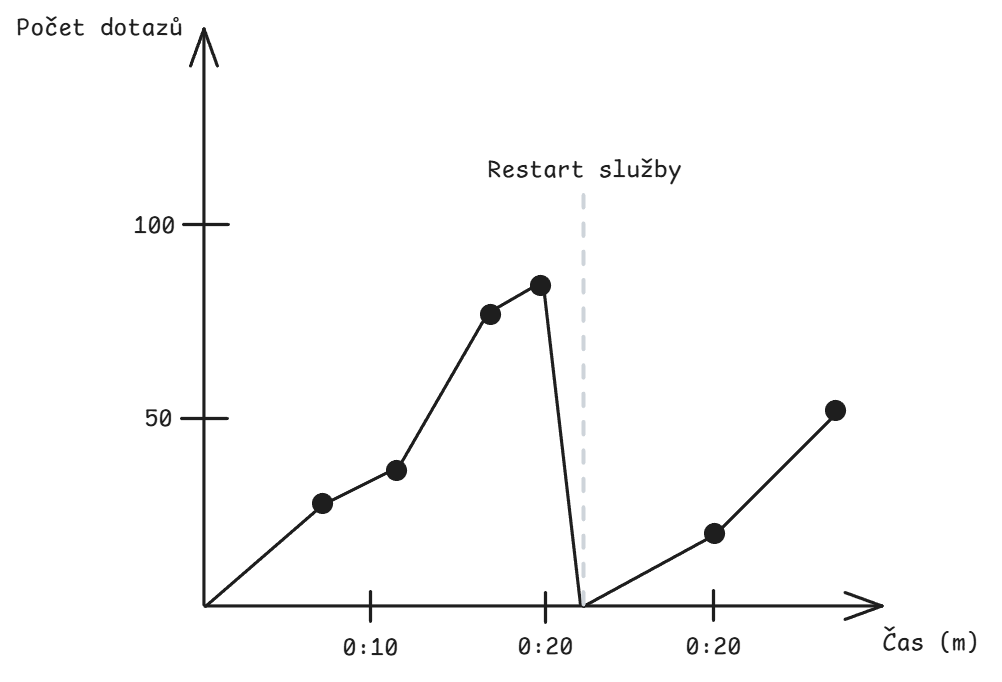
\includegraphics[width=0.8\textwidth]{images/counter.png}
        \caption{Ukázka metriky typu Counter}
        \label{fig:counter}
    \end{figure}
    \item \textbf{Gauge} \\ 
    Hodnota, která může růst i klesat, například aktuální využití CPU.
    \begin{figure}[H]
        \centering
        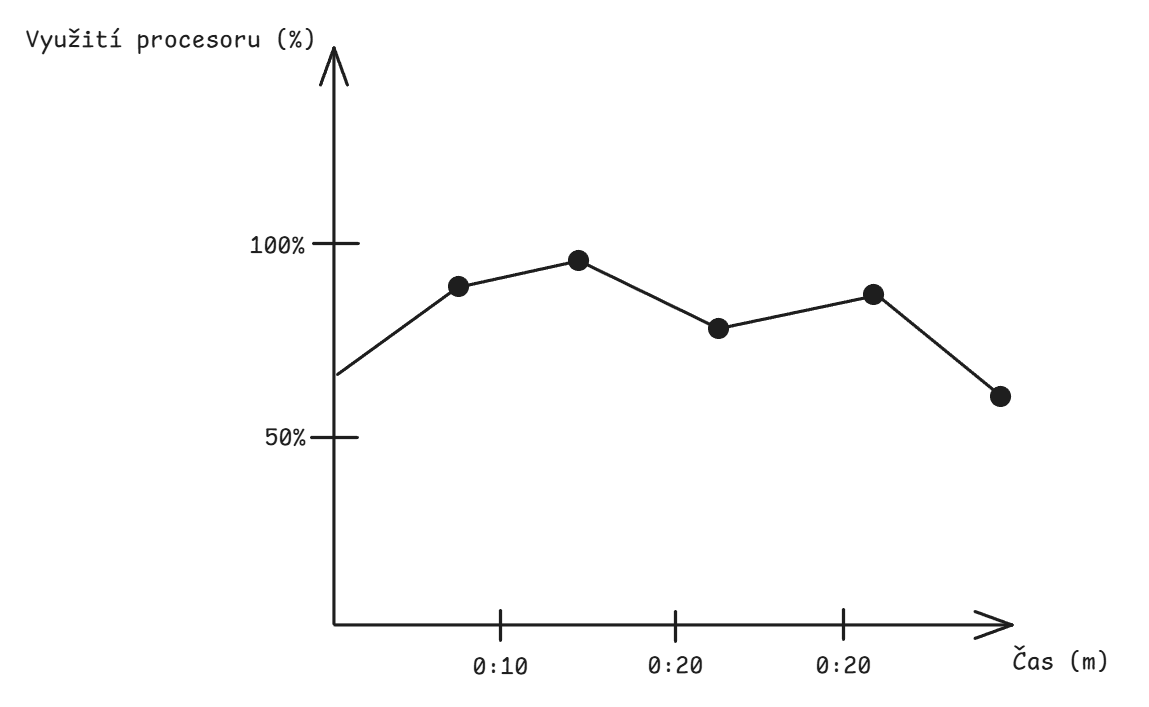
\includegraphics[width=0.8\textwidth]{images/gauge.png}
        \caption{Ukázka metriky typu Gauge}
        \label{fig:gauge}
    \end{figure}    
    \item \textbf{Histogram} \\
    Měří distribuci hodnot, například doby odezvy, a poskytuje informace o počtu vzorků a součtech pro různé intervaly.
    \begin{figure}[H]
        \centering
        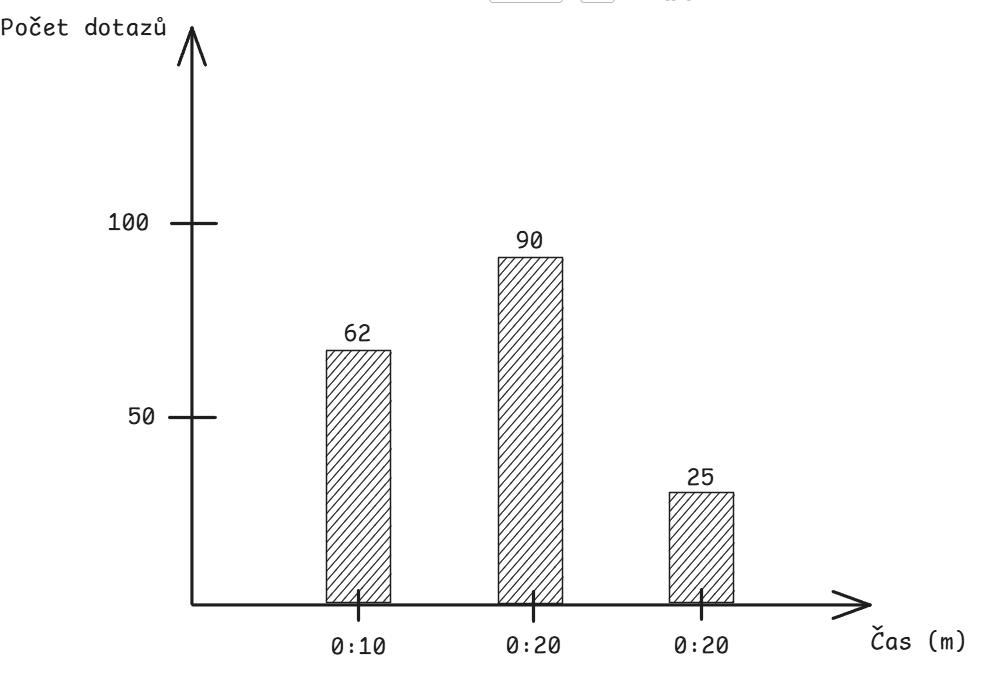
\includegraphics[width=0.8\textwidth]{images/histogram.png}
        \caption{Ukázka metriky typu Histogram}
        \label{fig:histogram}
    \end{figure}
    \item \textbf{Summary} \\ 
    Podobný histogramu, ale poskytuje kvantily pro měření distribuce, například 95. percentil doby odezvy.
\end{itemize}   

\subsubsection{PromQL}
PromQL, celým názvem Prometheus Query Language, je dotazovací jazyk pro Prometheus.
Dotazy mohou být buď "instantní", které vracejí aktuální hodnoty metrik, nebo "časový rozsah", které vracejí historické hodnoty pro zadané časové období. \cite{prometheusdocs}
\begin{lstlisting}[language=promql, caption={PromQL - ukázka dotazů}, label={lst:promql}, captionpos=b]
    rate(http_requests_total[5m])[30m:1m]
\end{lstlisting}
Tento dotaz vrací rychlost změny metriky \texttt{http\_requests\_total} za posledních 5 minut, přičemž se tato rychlost počítá pro každou minutu v posledních 30 minutách.

\subsubsection{Node Exporter}
Node Exporter je nástroj pro sběr systémových metrik z hostitelského systému, který je monitorován pomocí Prometheus.
Node Exporter shromažďuje informace o specifickém systému pro který je konfigurován, například o CPU, paměti, disku, síti a dalších hardwarových a systémových parametrech. \cite{prometheusdocs}

Je třeba ho distribuuovat a spustit na každém hostitelském systému, který chceme monitorovat, a poté nakonfigurovat Prometheus, aby shromažďoval data z těchto Node Exporterů. \cite{prometheusdocs}
\subsubsection{Alertmanager}
Alertmanager je komponenta Prometheus, která se stará o správu a odesílání upozornění.
Umožňuje definovat pravidla pro upozornění, která se spouštějí na základě dotazů PromQL, a poté odesílat upozornění prostřednictvím různých kanálů, jako jsou e-mail, Slack a další. \cite{prometheusdocs}
\subsection{Grafana}
Grafana je open-source platforma pro vizualizaci a analýzu dat, která umožňuje vytvářet interaktivní dashboardy a grafy z různých datových zdrojů.
Grafana podporuje širokou škálu datových zdrojů, včetně databází, časových řad, cloudových služeb a dalších, což umožňuje uživatelům snadno integrovat a vizualizovat data z různých systémů. \cite{grafanadocs}

Grafana byla původně vyvinuta v roce 2014 Torkel Ödegaardem jako větev projektu Kibana.
Nyní je Grafana Labs, společnost založená v roce 2015, hlavním vývojářem a správcem projektu.
\begin{figure}[h]
    \centering
    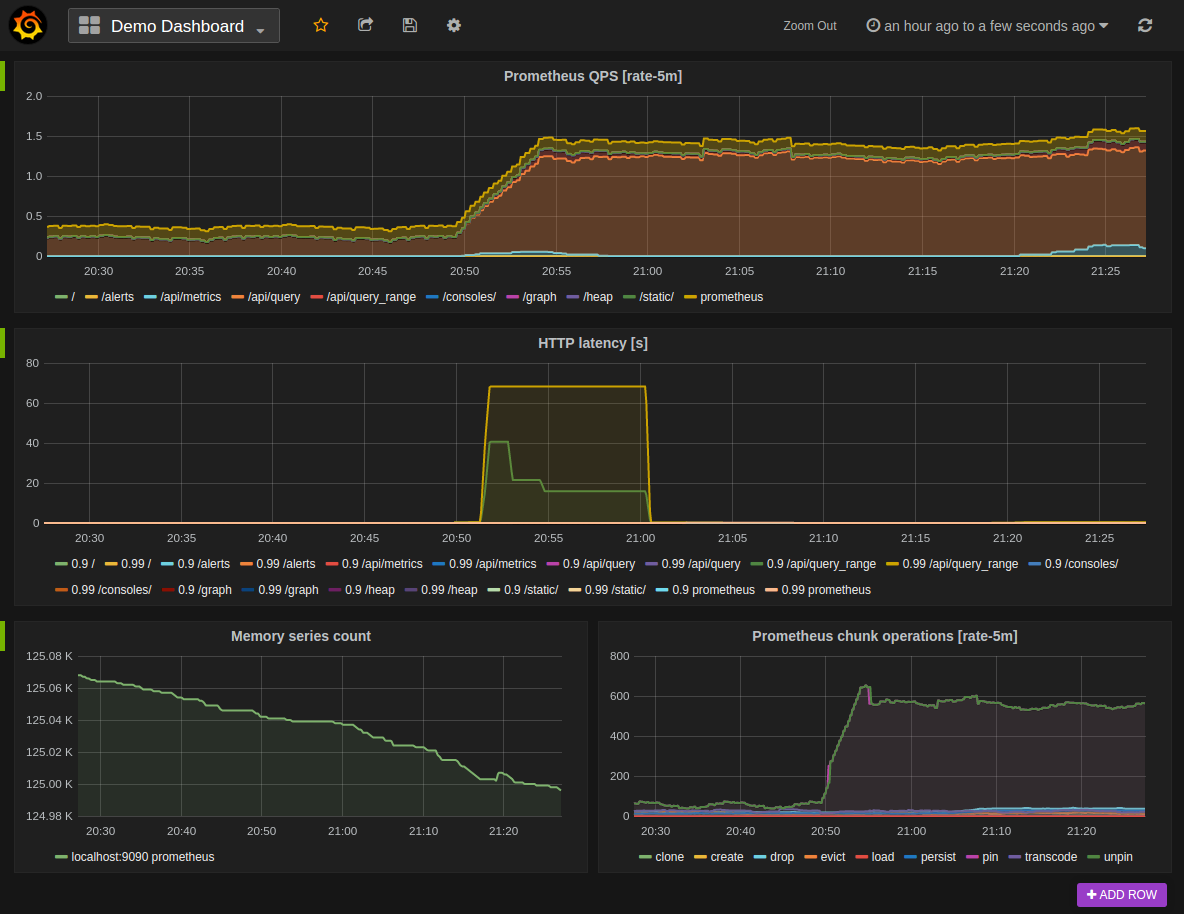
\includegraphics[width=0.8\textwidth]{images/grafana_prometheus.png}
    \caption{Ukázka dashboardu v Grafaně \cite{grafanadocs}}
    \label{fig:grafana}
\end{figure}

Grafana poskytuje vestavěnou podporu pro širokou škálu datových zdrojů, jako jsou například Prometheus, InfluxDB, Grafana Loki, SQL databáze a další. \cite{grafanadocs}
Dále je tu možnost přidat i vlastní datové zdroje pomocí pluginů. \cite{grafanadocs}

\subsubsection{Vizualizace}
Než může Grafana data vizualizovat, musí být nejprve dotazována na data z připojených datových zdrojů.
Na tyto zdroje se připojí pomocí tzv. pluginů, které umožňují jak komunikaci, tak konvert dat z příchozího formátu (JSON, CSV...) do
formátu, který Grafana dokáže zpracovat. Takový formát se nazyvá \textit{data frame}. \cite{grafanadocs}

Interní struktura takového data framu vypadá jako tabulka, kde každý sloupec představuje jednu proměnnou a každý řádek představuje jeden záznam.
\begin{table}[ht!]
\centering
\begin{tabular}{||c | c||} 
    \hline
    \textbf{time} & \textbf{temperature} \\ [0.5ex] 
    \hline\hline
    2024-05-05 10:22:24 & 43.0 \\ 
    \hline
    2024-05-05 10:22:25 & 45.3 \\
    \hline
    2024-05-05 10:22:26 & 44.4 \\
    \hline
    2024-05-05 10:22:27 & 41.2 \\
    \hline
    2024-05-05 10:22:28 & 49.7 \\
    \hline
    2024-05-05 10:22:29 & 67.0 \\
    \hline
\end{tabular}
\caption{Grafana - ukázka data framu teploty CPU}
\label{table:3}
\end{table}

Pokud by pro různá data bylo časové razítko stejné, Grafana je dokáže sloučit do jednoho data framu, což umožňuje například porovnávat různé metriky v čase. \cite{grafanadocs}

Následně se vytvoří dotazy, které vybírají konkrétní data z data framu. Tyto dotazy jsou psány v jazyce specifickém pro daný datový zdroj, například PromQL pro Prometheus. \cite{grafanadocs}
Nakonec se z dat vrácených dotazem vytvoří panel. Panel je kontejner pro vizualizaci dat, který může být různých typů, například graf, tabulka, text nebo mapa. \cite{grafanadocs}
Každý panel může být nakonfigurován tak, aby zobrazoval data určitým způsobem, například pomocí různých barev, os nebo legend. \cite{grafanadocs}

\section{Testování}

Testování výkonu a spolehlivosti softwarových systémů představuje nedílnou součást návrhu,
vývoje a provozu moderních aplikací. Jeho hlavním cílem je systematicky ověřit chování systému
při různých úrovních a typech zátěže, identifikovat úzká hrdla, vyhodnotit stabilitu a zajistit,
aby systém splňoval požadavky kladené reálným provozem.

V testování můžeme definovat několik klíčových odvětví:
\begin{itemize}
    \item \textbf{Spolehlivost} \\
    Typickými příklady spolehlivosti jsou:
        \begin{itemize}
            \item aplikace funguje tak, jak uživatel učekává
            \item dokáže tolerovat chyby uživatele
            \item výkon je dostatečně dobrý pro vyžadované použití, pod očekávaným zatížením
            \item dokáže zabránit neoprávněnému přístupu a využívání
        \end{itemize}
    Pokud jsou všechny tyto body splněny, můžeme říci, že systém je spolehlivý. \cite{kleppmann2017designing}
    
    Kvalitním nástrojem jak testovat spolehlivost jsou například chaos testy, které záměrně způsobují poruchy v systému, aby se ověřilo, zda dokáže správně reagovat a zotavit se z nich.
    Jedním takovým nástrojem je Chaos Monkey od Netflixu, který náhodně vypíná instance v produkčním prostředí, aby otestoval odolnost systému vůči selhání. \cite{chaosmonkeydocs}

    \item \textbf{Škálovatelnost} \\
    Škálovatelnost se týká schopnosti systému růst nebo zmenšovat své zdroje v závislosti na zátěži. Systém musí být schopen efektivně zpracovávat rostoucí množství požadavků bez výrazného snížení výkonu.

    Zátěž je ovšem ale více než jen počet požadavků. Může zahrnovat i různé typy zátěže, jako jsou například:
    \begin{itemize}
        \item dotazy za sekundu
        \item poměr čtení a zápisu
        \item současní aktivní uživatelé
    \end{itemize}

    Také je důležité identifikovat, kde se nacházejí úzká hrdla systému, která mohou omezovat jeho škálovatelnost.
    V jednom systému mohou být problém celkové průměrné zvednutí uživatelů, ale v jiném systému může být extrémní nárůst uživatelů v určité období - odlehlé hodnoty. \cite{kleppmann2017designing}
    
    \item \textbf{Výkon} \\
    V oblasti výkonu jsou dvě klíčové otázky, které je třeba zodpovědět:
    \begin{itemize}
        \item Když se zvedne zátěž, ale systémové zdroje zůstávají stejné, jak to ovlivní výkon?
        \item Když se zvedne zátěž, o kolik musíme zvednout systémové zdroje, aby výkon zůstal stejný?
    \end{itemize}

    V systémech které zpracovávají data se často bavíme o propustnosti, která udává, kolik dat je systém schopen zpracovat za jednotku času.
    V online systémech zase o výkonu často mluvíme v souvislosti s latencí, která udává, jak dlouho trvá zpracování jednotlivého požadavku. \cite{kleppmann2017designing}
\end{itemize}

Databázových systémů se týkají všechny tyto aspekty, a proto je důležité je testovat a porovnávat, aby bylo možné vybrat ten nejvhodnější pro konkrétní použití.

\subsection{Benchmarking a porovnávání systémů}

Benchmarking je metodický přístup k porovnávání výkonnosti různých systémů za definovaných a
reprodukovatelných podmínek. Cílem je zajistit objektivní srovnatelnost výsledků a eliminovat
vlivy okolního prostředí, které by mohly měření zkreslit.

V oblasti databázových systémů se benchmarking využívá například pro porovnání různých
datových struktur a úložných strategií, jako jsou B-Tree a LSM stromy. \cite{kleppmann2017designing}.

Klíčovým faktorem benchmarkingu je definice workloadu, který musí odpovídat reálnému použití
systému. Nevhodně zvolený scénář může vést k výsledkům, které neodrážejí skutečné chování
aplikace.

\subsubsection{B-Tree}
B-Tree je datová struktura, která uchovává data ve formě klíč-hodnota, která jsou seřazené podle klíče.

B-Tree rozdělí úložiště dat do několika fixních bloků (často odpovídajících velikosti diskového sektoru).
Každý takový blok může být lehce identifikovaný pomocí adresy a jeden blok může více adres odkazujících na jiné bloky. \cite{kleppmann2017designing}
Jeden blok je označený za kořenový blok, který je vždy výchozím bodem pro hledání dat.

\begin{figure}[H]
    \centering
    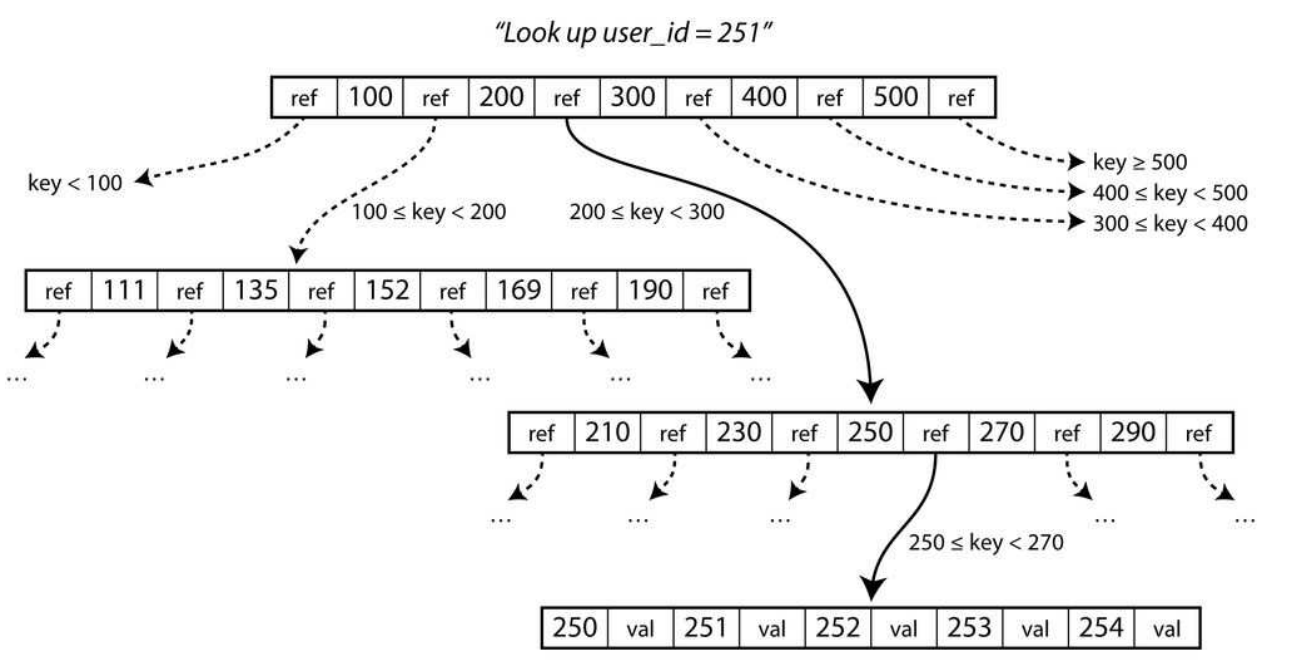
\includegraphics[width=0.8\textwidth]{images/b-tree_example.png}
    \caption{Ukázka organizace dat v B-Tree struktuře \cite{kleppmann2017designing}}
    \label{fig:btree}
\end{figure}

V ukázce na obrázku \ref{fig:btree} hledáme záznam s klíčem 251, takže víme, že musíme sledovat odkaz do seznamu 200-299.
Takový seznam se dále dělí do bloků seřazené od x-209, 210-229, 230-249, 250-269, 270-289 a 290-x.
Eventuelně se dostaneme až do správného bloku který hledáme. \cite{kleppmann2017designing}

\subsubsection{LSM Strom}
Log-Structured Merge-Tree je datová struktura optimalizovaná pro vysokou propustnost zápisů.
Každý zápis se nejprve uloží do rychlé paměti (memtable) a periodicky se přepíše do trvalého úložiště (disku) ve formě seřazených souborů (SSTables).
Tyto SSTables jsou přirozené seřazené podle klíče a je už dále neměnný. \cite{kleppmann2017designing}

Při čtení se pak postupuje nejdříve přečtením memtables a následně od nejnovějších SSTables k nejdřívějším, dokud se nenajde požadovaný záznam nebo se nedojde na konec. \cite{kleppmann2017designing}

\begin{figure}[H]
    \centering
    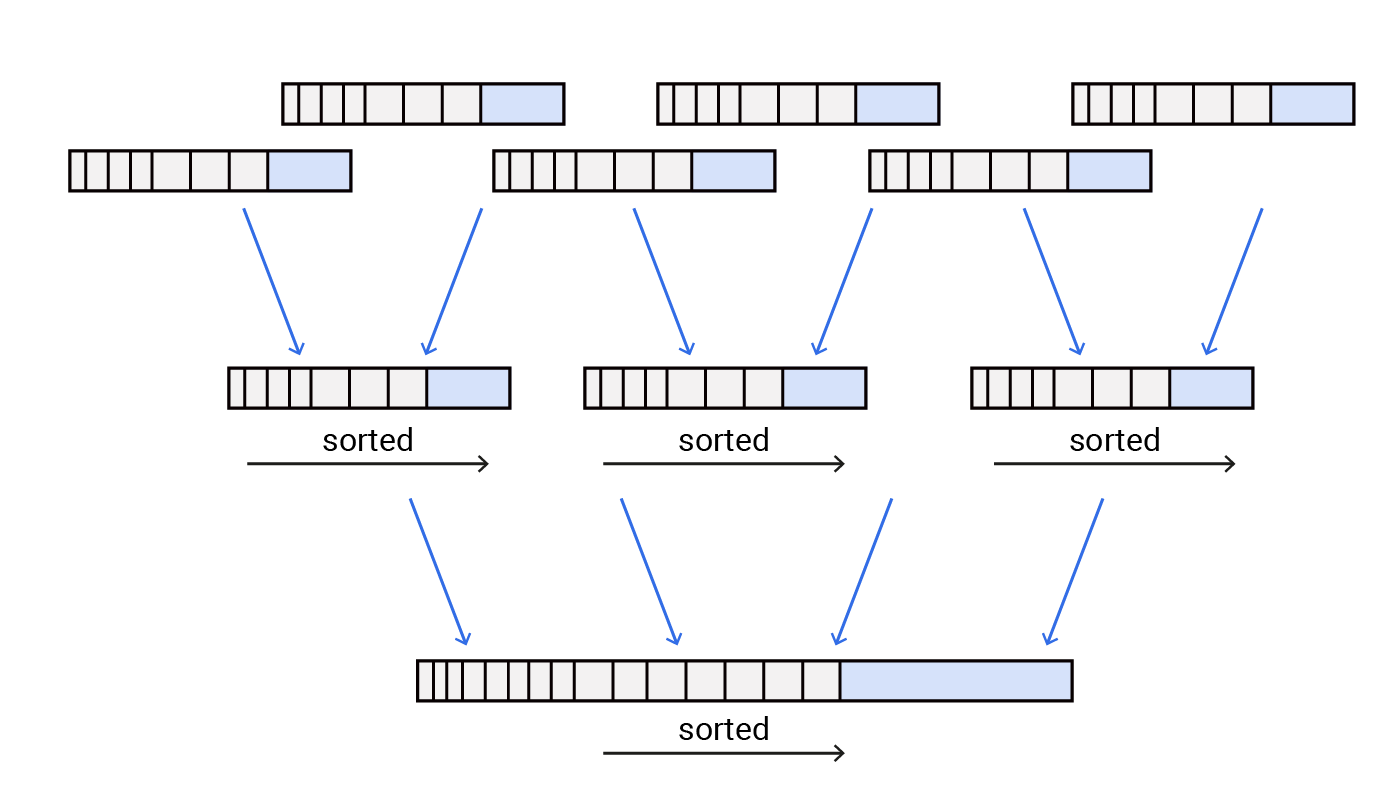
\includegraphics[width=0.8\textwidth]{images/lsmtree_example.png}
    \caption{Ukázka organizace dat v LSM stromu \cite{lsmtree}}
    \label{fig:lsmtree}
\end{figure}

Starší SSTables jsou pravidelně slučovány do větších souborů, aby se snížil počet souborů, které je třeba prohledávat při čtení, a aby se odstranily záznamy, které byly aktualizovány nebo smazány. \cite{kleppmann2017designing}
Díky tomu že jsou přirozeně seřazené, je tento proces slučování efektivní. \cite{kleppmann2017designing}

%\pagebreak
